\documentclass[12pt, dvipsnames, a4paper]{article}
\usepackage{geometry}
\geometry{legalpaper, margin=0.5in}
\usepackage{xcolor}
\usepackage{lipsum,etoolbox}
\usepackage{xspace} 
\usepackage[normalem]{ulem}
\usepackage{vwcol}
\usepackage{cancel}
\usepackage{enumitem}
\usepackage{amsmath}
\usepackage{caption}
\usepackage{graphicx}
\usepackage{amsfonts}
\usepackage{float}
\usepackage{multicol}
\usepackage{hyperref}
\usepackage{listings}
\usepackage{textcomp}
\usepackage{lstautogobble}
\usepackage[parfill]{parskip}
\usepackage{tikz-qtree}
\usepackage{tikz}
\usepackage{hyperref}
\usetikzlibrary{decorations.pathreplacing}
\tikzset{every tree node/.style={minimum width=4cm,draw,circle},
         blank/.style={draw=none},
         edge from parent/.style=
         {draw,edge from parent path={(\tikzparentnode) -- (\tikzchildnode)}},
         level distance=1.5cm}

%% Genearl %%
\renewcommand{\thesection}{\arabic{section}}


%% For convenience %%
\newcommand{\code}[1]{\texttt{#1}}
\newcommand{\bcode}[1]{\texttt{\textbf{#1}}}
\newcommand{\balert}[1]{\textbf{\alert{#1}}}
\newcommand{\rarrow}{$\Rightarrow$}
\newcommand{\tab}[1][0.5cm]{\hspace*{#1}}
\newcommand{\deepemphasis}[1]{\underline{\textbf{\Large{#1}}}}
\newcommand{\bfemph}[1]{\textbf{\emph{#1}}}
\newcommand{\OR}[0]{\lvert \: \rvert}

%% Colours %%
\definecolor{mLightBrown}{HTML}{EB811B}
\definecolor{mLightGreen}{HTML}{14B03D}

%% Pseudocode %% 
\lstdefinelanguage{pseudo}
{
	keywords=[1]{
		let,
		class,
		new,
		loop,
		until,
		end,
		if,
		else,
		then,
		return,
		while,
		for,
		to,
		fun,
		break,
		and,
		true,
		false,
		or,
		do,
		max,
		min,
		elif,
	},
	keywordstyle=[1]\color{black}\bf,
	keywords=[2] {
		invariant,
		precond,
		postcond
	},
	keywordstyle=[2]\color{blue}\bf
}

\lstset{
	breaklines		=	true,
	language 		= 	pseudo,
	basicstyle		=	\ttfamily,
	mathescape		=	true,
	escapeinside	=	||,
	tabsize			=	2,
	numbers			=	left,
	commentstyle	=	\color{OliveGreen},
	stringstyle		=	\color{mLightBrown},
	upquote			=	true,
	morestring		=	[b]',
	moredelim		=	[l][\rmfamily\itshape]{@},
	comment			=	[l]{//},
	morecomment		=	[s]{/*}{*/},
	commentstyle=\color{Gray}\ttfamily,
	showstringspaces=	false,
	showtabs		=	false,
	autogobble
}

%% Other %%
\setcounter{secnumdepth}{5}
\setcounter{tocdepth}{5}

% \patchcmd{<cmd>}{<search>}{<replace>}{<success>}{<failure>}
\patchcmd{\abstract}{\titlepage}{\titlepage% Insert ToC-writing after starting a titlepage
  \addcontentsline{toc}{chapter}{Abstract}}{}{}
\setcounter{secnumdepth}{3}
\setcounter{tocdepth}{3}

% Keywords command
\providecommand{\keywords}[1]
{
  \small	
  \textbf{\textit{Keywords---}} #1
}


%**************************************************************************************************************%
%______________________________________________________________________________________________________________%
\begin{document}
\title{\textbf{EECS 4314 - Bit Theory\\Architecture Report}}
\date{\Large \today}
\author{
	\small \textbf{Amir Mohamad}\\ amohamad@my.yorku.ca\\\\
	\small \textbf{Arian Mohamad Hosaini}\\ mohama23@my.yorku.ca\\\\
	\small \textbf{Dante Laviolette}\\ dantelav@my.yorku.ca\\\\
	\small \textbf{Diego Santosuosso Salerno}\\ nicodemo@my.yorku.ca\\\\
	\small \textbf{Isaiah Linares}\\ isaiah88@my.yorku.ca\\\\
	\small \textbf{Misato Shimizu}\\\\
	\small \textbf{Muhammad Hassan}\\ furquanh@my.yorku.ca\\\\
	\small \textbf{Yi Qin}\\ aidenqin@my.yorku.ca\\\\
	\small \textbf{Zhilong Lin}\\ lzl1114@my.yorku.ca\\\\
	\small York University\\
}
\maketitle
\newpage
\hspace{0pt}
\vfill
\begin{abstract}
	\lipsum[1]
	\lipsum[1]
	\\\\
	\keywords{keyword1, keyword2, keyword3}
\end{abstract}
\vfill
\hspace{0pt}
\newpage
\tableofcontents
\clearpage

\section{How to use \LaTeX}
\subsection{Basics}
\textbf{bold text} dolor sit amet. Inline math $\sum_{0}^{\inf} x$. Bold inline math $\mathbf{\sum_{0}^{\inf} x}$ consectetuer adipiscing elit. Ut purus elit, vestibulum ut, placerat ac, adip-
iscing vitae, felis. \emph{Emphasized text}. \textbf{\emph{Emphasized bold text}} curabitur dictum gravida mauris. Nam arcu libero, nonummy eget, consectetuer id,
vulputate a, magna. Donec vehicula augue eu neque. Pellentesque habitant morbi tristique senectus et
netus et refering to code \code{JavaClass.java}. \textbf{\code{BoldJavaClass.java}} fames ac turpis egestas. Mauris ut leo. Cras viverra metus rhoncus sem. Nulla et lectus
vestibulum urna fringilla ultrices. Phasellus eu tellus sit amet tortor gravida placerat. Integer sapien est,
iaculis in, pretium quis, viverra ac, nunc. Praesent eget sem vel leo ultrices bibendum. Aenean faucibus.
Morbi dolor nulla, malesuada eu, pulvinar at, mollis ac, nulla. Curabitur auctor semper nulla. Donec
varius orci eget risus. Duis nibh mi, congue eu, accumsan eleifend, sagittis quis, diam. Duis eget orci sit
amet orci dignissim rutrum. Update tutorial file. Block equations:
\begin{equation}
	\int_\alpha^\beta f'(x) \, dx=f(\beta)-f(\alpha).
\end{equation}
We can use the fundamental theorem of calculus to say that
$\int_2^3 x^2 \, dx=\frac{3^3}{3}-\frac{2^3}{3}=\frac{19}{3}$.
Also note that $\displaystyle \int_2^3 x^2 \, dx=\frac{3^3}{3}-\frac{2^3}{3}=\frac{19}{3}$.
We can also give this equation its own line
\[
	\int_2^3 x^2 \, dx=\frac{3^3}{3}-\frac{2^3}{3}=\frac{19}{3}.
\]

\subsection{Pseudocode}
\begin{lstlisting}[frame=single, basicstyle=\small]
precond graph1 and graph2 $[(i_1,j_1),..,(i_{k<=m},j_{k<=m})]$
precond $\code{graph1.length} = k_1$
precond $\code{graph2.length} = k_2$
precond $n$ is number of nodes
precond $m$ is max number of edges
precond $p >= n^2$
precond $\code{graph}[k].ij$ is the integer concat of edge $k: (i,j)$

fun isSubGraph($\code{graph1}, \code{graph2}$)
	precond $h: \text{edge } (i,j): ij \in \mathbb{Z} \longrightarrow k \in {0,\dots,m-1}$
	let $h$ be the hash function defined by $h(x) = (x \text{ mod } p) \text{ mod } m$
	let $B[0\dots m - 1]$ be an array of linked lists; initially all lists are empty
	
	// we will hash the second graph
	for k $\longleftarrow 0\dots \code{graph2.length}$	
		iterate across $B[h(\code{graph2}[k].ij)]$ looking for $\code{graph2}[k].ij$
 		if found, stop and throw error
		else append $\code{graph2}[k].ij$ to the list $B[h(\code{graph2}[k].ij)]$
 		end if
	end for

	// loop graph1 edges and return false if edge not in $B$
	for k $\longleftarrow 0\dots \code{graph1.length}$	
		iterate across $B[h(\code{graph1}[k].ij)]$ looking for $graph1[k].ij$
 		if found, continue
		else return false postcond graph1 is not a subgraph
 		end if
	end for

	postcond $B$ contained all the edges of graph1	
	return true
\end{lstlisting}
\clearpage
\subsection{Insert Images with Figures}
\begin{figure}[hbt!]
	\caption{Demo image of a basic OS architecture}
	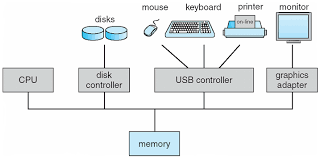
\includegraphics[scale=.8]{assets/demo.png}
	\centering
\end{figure}
\subsection{Lists}
Lists are easy to create:
\begin{itemize}
	\item List entries start with the \verb|\item| command.
	\item Individual entries are indicated with a black dot, a so-called bullet.
	\item The text in the entries may be of any length.
	\item Latex is awesome! -Arian
\end{itemize}
Numbered (ordered) lists are easy to create:
\begin{enumerate}
	\item Items are numbered automatically.
	\item The numbers start at 1 with each use of the \texttt{enumerate} environment.
	\item Another entry in the list
\end{enumerate}

\section{Section}
\lipsum[1]
\subsection{SubSection}
\lipsum[1]
\subsubsection{SubSubSection}
\lipsum[1]

\begin{thebibliography}{00}
	\bibitem{b2} Clarke, Arthur C. 2001: A Space Odyssey. New York: Roc, 1968. 297.
\end{thebibliography}
\end{document}
